\documentclass[conference]{IEEEtran}
\IEEEoverridecommandlockouts
\usepackage{cite}
\usepackage{amsmath,amssymb,amsfonts}
\usepackage{algorithmic}
\usepackage{graphicx}
\usepackage{textcomp}
\usepackage{xcolor}
\usepackage{booktabs}
\usepackage{array}
\def\BibTeX{{\rm B\kern-.05em{\sc i\kern-.025em b}\kern-.08em
    T\kern-.1667em\lower.7ex\hbox{E}\kern-.125emX}}
\begin{document}

\title{Regime-Dependent Cross-Sectional Predictability in US Equities:\\
A Comparison of LSTM and Classical Machine Learning}

\author{\IEEEauthorblockN{Nicholas Hong}
\IEEEauthorblockA{\textit{School of Electrical and Electronic Engineering} \\
\textit{Nanyang Technological University}\\
Singapore \\
}}

\maketitle

\begin{abstract}
We evaluate whether Long Short-Term Memory (LSTM) networks outperform classical
machine learning for forecasting daily United States equity returns, using a
panel of 518 S\&P 500 constituents spanning March 2005 to July 2026 sourced from
Bloomberg. Under a strictly chronological protocol with an explicit shuffled-target
leakage control, we find that no model, LSTM included, predicts next-day return
\emph{levels} with an accuracy exceeding a naive zero-return baseline. Reframing
the task cross-sectionally, that is, predicting which stocks will out- or
under-perform the daily universe mean, reveals statistically significant
predictability that is concentrated in high-volatility regimes: a gradient-boosted
tree attains a mean daily rank information coefficient (IC) of 0.044 ($t=3.2$) on
high-volatility days versus 0.005 ($t=0.9$) on calm days, and the nonlinear model
overtakes linear models specifically under stress. However, this predictability
is a one-day phenomenon. A decile long-short portfolio earns a gross annualized
Sharpe ratio of 2.09 in high-volatility periods but does not survive transaction
costs at daily rebalancing (net Sharpe negative for every configuration), and the
signal decays to an information coefficient of approximately zero at a five-day
horizon, so slower rebalancing removes both the cost and the edge. We conclude
that the detectable structure is a short-horizon, stress-concentrated effect that
is real but not economically exploitable at the frequencies studied, and we argue
that this negative-but-rigorous result is the appropriate scientific conclusion
for the setting.
\end{abstract}

\begin{IEEEkeywords}
LSTM, machine learning, equity return forecasting, cross-sectional momentum,
market regimes, transaction costs, information coefficient
\end{IEEEkeywords}

\section{Introduction}
Deep learning has been widely proposed for financial time-series forecasting, and
recurrent architectures such as the LSTM \cite{hochreiter1997} are natural
candidates given the sequential structure of price data. A recurring difficulty in
this literature is that daily equity returns are close to a martingale difference
sequence: their conditional mean is small relative to their volatility, and simple
benchmarks are hard to beat out-of-sample \cite{gu2020,depradombook}. Reported
successes frequently arise from subtle look-ahead leakage, survivorship bias, or
evaluation that ignores transaction costs.

This paper asks a deliberately narrow question with a rigorous answer: on a broad,
recent panel of US large-capitalization equities, does an LSTM provide any edge
over classical machine learning for daily return prediction, and if any signal
exists, is it economically meaningful? Our contribution is threefold. First, we
establish that daily return-\emph{level} prediction is a null result across eleven
model families including an LSTM, validated by a shuffled-target control that
confirms the absence of leakage. Second, we show that a cross-sectional
reformulation uncovers genuine, statistically significant predictability that is
concentrated in high-volatility regimes and is stronger for nonlinear models.
Third, through a horizon-and-cost analysis we demonstrate that the effect is a
one-day phenomenon that survives neither transaction costs at daily frequency nor
the passage of time to a weekly horizon. The result is a complete characterization
of where the signal lives and why it is not tradeable.

\section{Related Work}
Fischer and Krauss \cite{fischer2018} apply LSTMs to S\&P 500 constituents and
report profitability before costs, while Krauss \emph{et al.} \cite{krauss2017}
study deep networks and gradient boosting for statistical arbitrage. Gu, Kelly and
Xiu \cite{gu2020} provide a comprehensive empirical asset-pricing benchmark and
emphasize that tree ensembles and neural networks capture cross-sectional rather
than time-series structure. The short-horizon reversal effect we ultimately
isolate is consistent with the microstructure and liquidity-provision literature
\cite{lo1990}, in which apparent short-term predictability is compensation for
bearing inventory risk and is eroded by trading frictions. Our methodological
posture, in particular the emphasis on point-in-time data, chronological
validation and explicit leakage tests, follows de Prado \cite{depradombook}.

\section{Data}
The dataset comprises daily open, high, low, close and volume observations for the
S\&P 500 membership, exported from a Bloomberg Terminal via a custom staged
export pipeline. After cleaning, the panel contains 2{,}448{,}678 stock-day
observations across 518 tickers from March 2005 to July 2026. Prices are
unadjusted terminal fields; corporate-action treatment is discussed in Section
\ref{sec:limitations}. A parallel context dataset of twelve macro-financial series
(equity indices, the VIX and MOVE volatility indices, the dollar index, the 2-,
10- and 30-year Treasury yields, and front-month crude oil, gold and copper) is
used for regime definition and auxiliary features.

To keep development independent of terminal access, an open-source mirror was
built from public sources with an identical output schema, and a parity check
against the Bloomberg closes gave a median absolute difference of essentially zero
across overlapping tickers, with the few larger discrepancies attributable to
corporate-action conventions.

\section{Methodology}

\subsection{Features and Target}
All predictive features are constructed from information available at the close of
day $t$. They include multi-horizon log returns (1, 5, 21 days), 21-day realized
volatility, an intraday high-low range, price-to-moving-average deviations, and a
log-volume $z$-score. For the cross-sectional task we additionally compute the
daily percentile rank of each momentum, volatility and volume feature across the
universe. Macro-context features (volatility-index levels and changes, a Treasury
term spread, and commodity momentum) are appended by trading date.

The level target is the next-day log return, $r_{i,t+1}$. The cross-sectional
target is the daily demeaned return,
\begin{equation}
\tilde{r}_{i,t+1} = r_{i,t+1} - \frac{1}{N_t}\sum_{j=1}^{N_t} r_{j,t+1},
\end{equation}
which isolates relative performance and is dollar-neutral by construction.

\subsection{Splits and Leakage Protocol}
Data are partitioned strictly chronologically: training through 2021, validation
in 2022, and testing from 2023 onward (466{,}426 test observations). Feature
scalers and all hyperparameters are fit on training and validation data only. As a
falsification test we retrain a representative model on \emph{shuffled} training
targets; a non-trivial out-of-sample IC in that setting would indicate leakage. The
control returns IC $=0.004$ ($t=0.67$), statistically indistinguishable from zero,
supporting the integrity of the pipeline.

\subsection{Models}
We compare eleven families: a zero-return and a momentum naive baseline; ordinary,
ridge and elastic-net linear regression; a decision tree, random forest, XGBoost
and LightGBM; a linear support-vector regressor; a degree-two polynomial ridge; and
an LSTM. The reported LSTM is a compact single-layer network (hidden size 32,
dropout 0.1) trained on 30-day sequences pooled across the panel with shared
weights, optimized with Adam under early stopping on validation loss (patience
two) and gradient clipping. A higher-capacity two-layer variant (hidden size 64,
dropout 0.2, patience five) was also trained; it reached a lower validation loss
but its test metrics were not retained, so no result is reported for it, and the
level-prediction conclusion below holds for both configurations. Tree and boosting
models use early stopping on the validation set; linear and kernel models are
standardized within a pipeline.

\subsection{Evaluation}
Beyond root-mean-square error and directional accuracy, our primary metric is the
mean daily cross-sectional rank IC, the Spearman correlation between predicted and
realized returns computed per day and averaged, with a $t$-statistic across days.
For the economic assessment we form a daily decile long-short portfolio, taking
equal-weighted long and short positions in the top and bottom prediction deciles.
We report gross and net annualized Sharpe ratios, maximum drawdown, and average
one-way turnover. Costs are charged at 10 basis points per side on the one-way
turnover $\sum_i |w_{i,t}-w_{i,t-1}|$ at each rebalance.

\section{Results}

\subsection{Daily Level Prediction is a Null Result}
Table \ref{tab:horserace} reports test-set performance for the level target. No
model materially beats the naive zero baseline on RMSE, and directional accuracy
sits near 50\% throughout. The strongest information coefficients belong to the
linear and support-vector models (IC $\approx 0.011$--$0.014$, $t\approx1.9$--$2.4$),
which are marginal, while the LSTM attains IC $=0.004$ ($t=0.76$), statistically
identical to the shuffled-target control. Gradient boosting and the decision tree
have negative point-estimate ICs. The headline conclusion is unambiguous: for
next-day return levels, an LSTM offers no advantage, and the task is effectively
unforecastable with these features.

\begin{table}[t]
\caption{Daily Level Prediction, Test Set (2023--2026)}
\label{tab:horserace}
\centering
\small
\begin{tabular}{@{}lrrr@{}}
\toprule
Model & Dir.\ Acc. & IC & IC $t$-stat \\
\midrule
SVR (linear)          & 0.490 & 0.0141 & 2.42 \\
Ridge / Linear        & 0.491 & 0.0109 & 1.86 \\
XGBoost               & 0.497 & 0.1413 & 1.83 \\
LSTM                  & 0.480 & 0.0042 & 0.76 \\
Shuffled-target (ctrl)& 0.498 & 0.0039 & 0.67 \\
Naive zero            & ---   & ---    & ---  \\
LightGBM              & 0.496 & $-0.0295$ & $-0.69$ \\
Decision tree         & 0.497 & $-0.0838$ & $-1.60$ \\
\bottomrule
\end{tabular}
\end{table}

\subsection{Cross-Sectional Predictability Concentrates in High-Volatility Regimes}
We define a high-volatility regime as any day on which the 63-day $z$-score of the
VIX exceeds one; this labels 18.7\% of days and uses only information through day
$t$. Table \ref{tab:xsregime} reports the cross-sectional results by regime. Two
findings stand out. First, predictability is strongly regime-dependent: LightGBM
achieves IC $=0.044$ ($t=3.2$) on high-volatility days against $0.005$ ($t=0.9$) on
normal days, and the pooled significance masks this concentration. Second, the
nonlinear model overtakes the linear model \emph{only} under stress, indicating
nonlinear cross-sectional structure that pays off when volatility is high. An
auxiliary experiment shows that the macro-context features contribute little beyond
the regime split itself: ridge attains a comparable high-volatility IC with and
without context, so it is the conditioning on regime, not the macro features, that
matters.

\begin{table}[t]
\caption{Cross-Sectional Daily Results by Regime, Test Set}
\label{tab:xsregime}
\centering
\small
\begin{tabular}{@{}llrrrr@{}}
\toprule
Model & Regime & IC & IC $t$ & Sharpe$_{\text{gr}}$ & Sharpe$_{\text{net}}$ \\
\midrule
Ridge    & high-vol & 0.0320 & 1.87 & 0.96 & $-0.69$ \\
Ridge    & normal   & 0.0111 & 2.04 & 0.28 & $-2.93$ \\
Ridge    & all      & 0.0154 & 2.76 & 0.48 & $-1.99$ \\
LightGBM & high-vol & 0.0436 & 3.17 & 2.09 & $-0.88$ \\
LightGBM & normal   & 0.0048 & 0.88 & $-0.24$ & $-4.89$ \\
LightGBM & all      & 0.0127 & 2.44 & 0.44 & $-3.55$ \\
\bottomrule
\end{tabular}
\end{table}

\subsection{The Signal is Short-Horizon and Not Cost-Survivable}
The gross portfolio results are economically striking: the LightGBM high-volatility
sleeve earns a gross annualized Sharpe of 2.09 with a shallow drawdown, and Fig.
\ref{fig:daily} shows its cumulative long-short return accruing almost entirely
within high-volatility windows. The effect nonetheless fails two independent tests
of economic reality. First, transaction costs eliminate it: average one-way daily
turnover is roughly 2.6, implying about 26 basis points of daily cost, which
exceeds the edge and drives every net Sharpe below zero (Table \ref{tab:xsregime}).
Second, the signal does not persist. Retargeting to a five-day forward return and
rebalancing weekly with non-overlapping observations collapses the high-volatility
IC to $-0.007$ (Table \ref{tab:weekly}); the gradient-boosted model degenerates to
near-constant predictions (best iteration 1, prediction standard deviation
$1.4\times10^{-4}$), finding no exploitable structure at that horizon. Slower
rebalancing therefore removes the cost burden and the signal simultaneously.

\begin{table}[t]
\caption{Five-Day Horizon, Weekly Rebalance (Non-Overlapping)}
\label{tab:weekly}
\centering
\small
\begin{tabular}{@{}llrrr@{}}
\toprule
Model & Regime & IC & IC $t$ & Sharpe$_{\text{net}}$ \\
\midrule
Ridge    & high-vol & $-0.0071$ & $-0.19$ & $-0.27$ \\
Ridge    & normal   & 0.0027    & 0.20    & $-0.74$ \\
Ridge    & all      & 0.0007    & 0.05    & $-0.64$ \\
LightGBM & all      & \multicolumn{3}{c}{degenerate (no splits)} \\
\bottomrule
\end{tabular}
\end{table}

\begin{figure}[t]
\centering
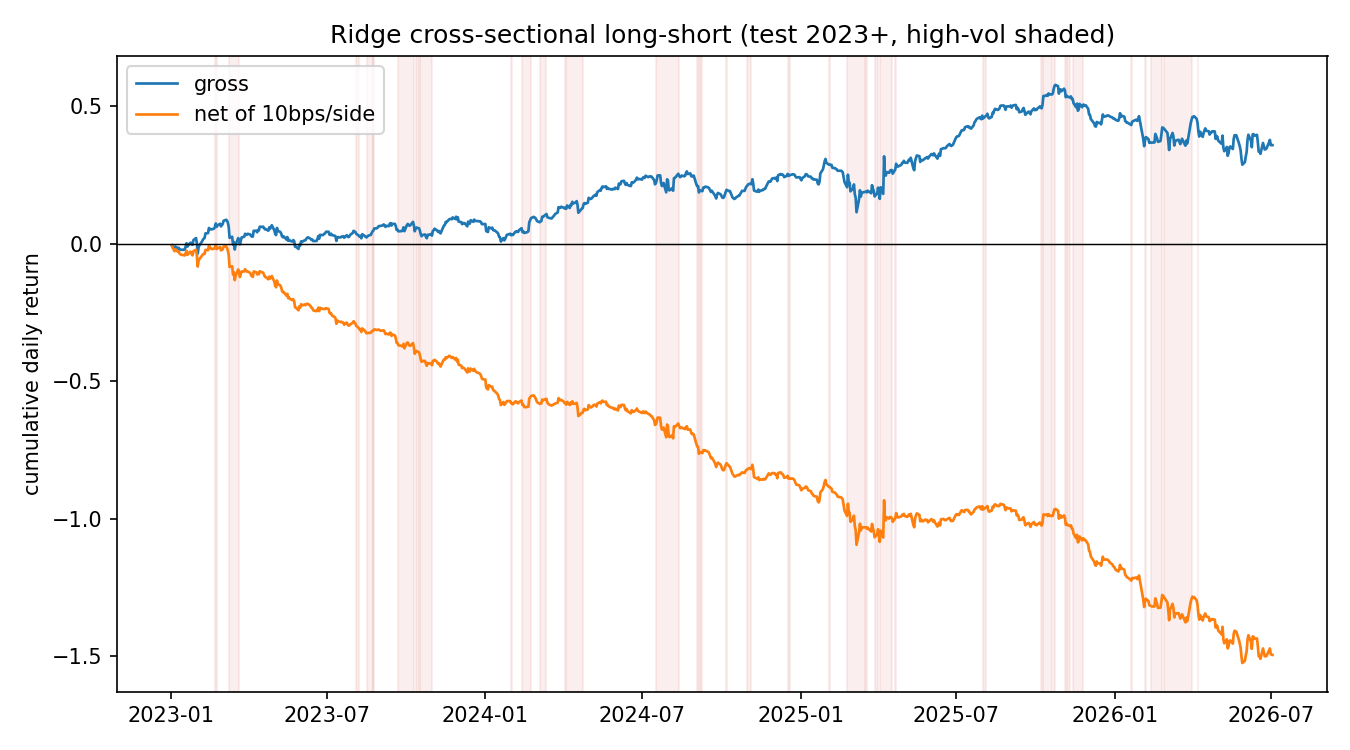
\includegraphics[width=\columnwidth]{xs_ls_equity_curve.png}
\caption{Cumulative daily cross-sectional long-short return for the ridge model on
the test set. Shaded bands mark high-volatility regimes. Gains accrue almost
exclusively during stress periods; the net-of-cost line is materially below the
gross line.}
\label{fig:daily}
\end{figure}

\section{Discussion and Limitations}
\label{sec:limitations}
The pattern we observe, short-horizon relative predictability that intensifies in
volatile markets and is competed away by trading costs, is consistent with
short-term reversal as compensation for liquidity provision \cite{lo1990}. Its
concentration in high-volatility regimes is intuitive: dispersion and the reward
for absorbing order-flow imbalance both rise with volatility.

Several limitations bound our claims. The universe is current-membership S\&P 500,
which introduces survivorship bias; because such bias typically \emph{flatters}
performance, the true exploitable edge is if anything smaller than reported, which
strengthens rather than weakens the negative economic conclusion. A point-in-time
membership reconstruction is the natural remediation. Prices use terminal fields
without total-return adjustment, and the cost model, though deliberately
conservative, is a stylized proxy for realistic execution. Finally, the study is
confined to one market and one signal family; whether the regime effect replicates
in other equity markets, and whether slower fundamental signals behave differently,
are questions for future work.

\section{Conclusion}
On a broad, recent panel of US equities we find that daily return-level prediction
is a null result for every model considered, an LSTM included, and that a
cross-sectional reformulation reveals statistically significant predictability that
is concentrated in high-volatility regimes and stronger for nonlinear models. That
predictability is nonetheless a one-day effect that survives neither transaction
costs at daily frequency nor the transition to a weekly horizon. The signal is
therefore real but not economically exploitable at the frequencies studied. We view
the value of the work as methodological as much as empirical: with careful
leakage controls, chronological evaluation and an explicit cost accounting, the
honest answer is a precisely characterized negative result, which is more credible
and more useful than an unaudited backtest that appears to succeed.

\begin{thebibliography}{00}
\bibitem{hochreiter1997} S. Hochreiter and J. Schmidhuber, ``Long short-term
memory,'' \emph{Neural Computation}, vol. 9, no. 8, pp. 1735--1780, 1997.
\bibitem{gu2020} S. Gu, B. Kelly, and D. Xiu, ``Empirical asset pricing via machine
learning,'' \emph{Review of Financial Studies}, vol. 33, no. 5, pp. 2223--2273,
2020.
\bibitem{fischer2018} T. Fischer and C. Krauss, ``Deep learning with long
short-term memory networks for financial market predictions,'' \emph{European
Journal of Operational Research}, vol. 270, no. 2, pp. 654--669, 2018.
\bibitem{krauss2017} C. Krauss, X. A. Do, and N. Huck, ``Deep neural networks,
gradient-boosted trees, random forests: Statistical arbitrage on the S\&P 500,''
\emph{European Journal of Operational Research}, vol. 259, no. 2, pp. 689--702,
2017.
\bibitem{lo1990} A. W. Lo and A. C. MacKinlay, ``When are contrarian profits due to
stock market overreaction?'' \emph{Review of Financial Studies}, vol. 3, no. 2,
pp. 175--205, 1990.
\bibitem{depradombook} M. L. de Prado, \emph{Advances in Financial Machine
Learning}. Hoboken, NJ: Wiley, 2018.
\end{thebibliography}

\end{document}
